\chapter{Kết quả}
\label{Chapter5}

\emph{Chương này trình bày kết quả đề tài, kết quả phát hiện intent, trích xuất thông tin và các chức năng đã cài đặt được.}

\section{Một số chức năng chính đã cài đặt}

\subsection{Chức năng chỉ đường từ một đia điểm đến một địa điểm xác định}
\begin{figure}[htp]
    \centering
    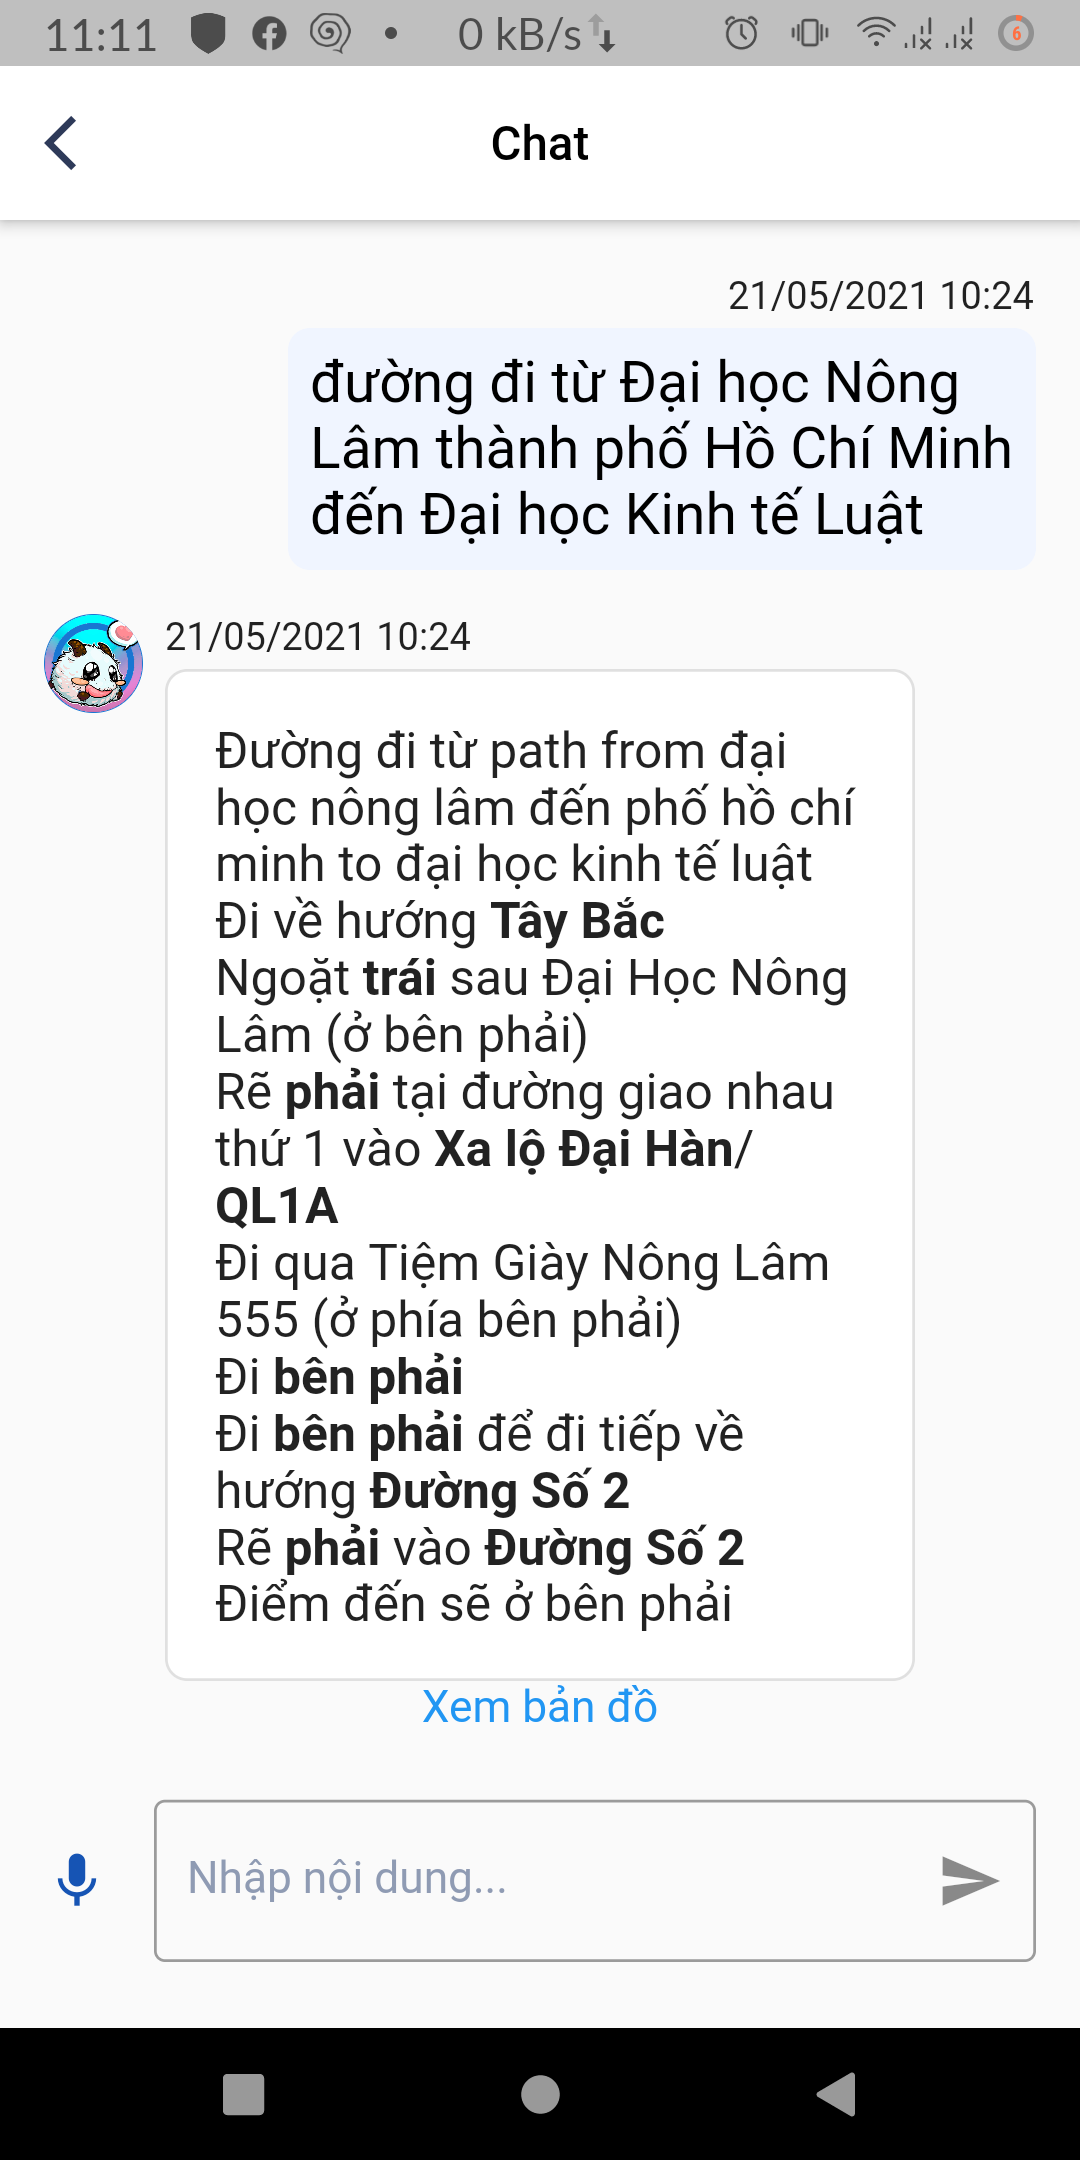
\includegraphics[width=10cm]{images/Screen-chat.png}
    \caption{Màn hình trò chuyện}
    \label{fig:screen-chat}
\end{figure}

\begin{figure}[htp]
    \centering
    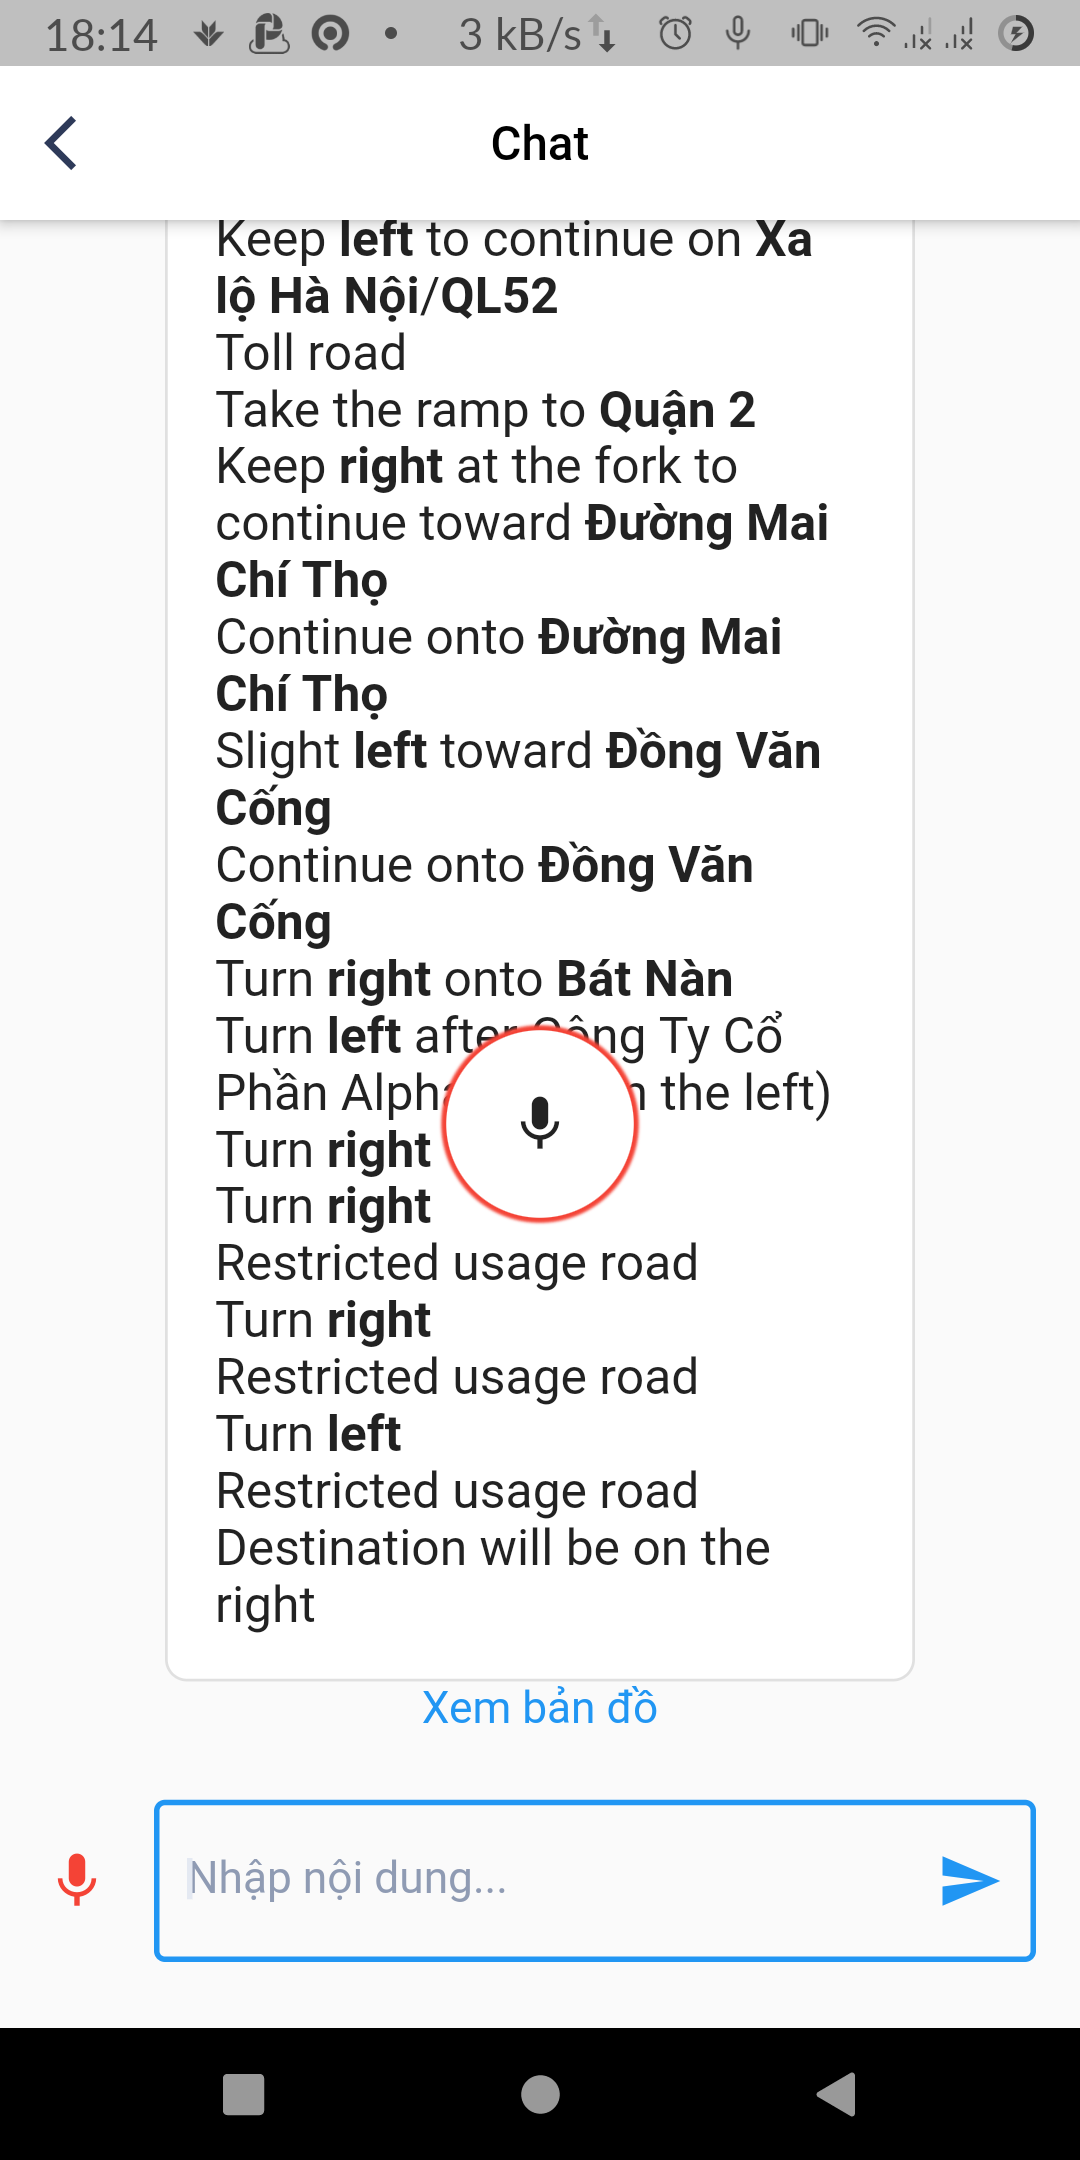
\includegraphics[width=10cm]{images/Screen-record.png}
    \caption{Màn hình thể hiện đang ghi âm}
    \label{fig:screen-record}
\end{figure}

\begin{figure}[htp]
    \centering
    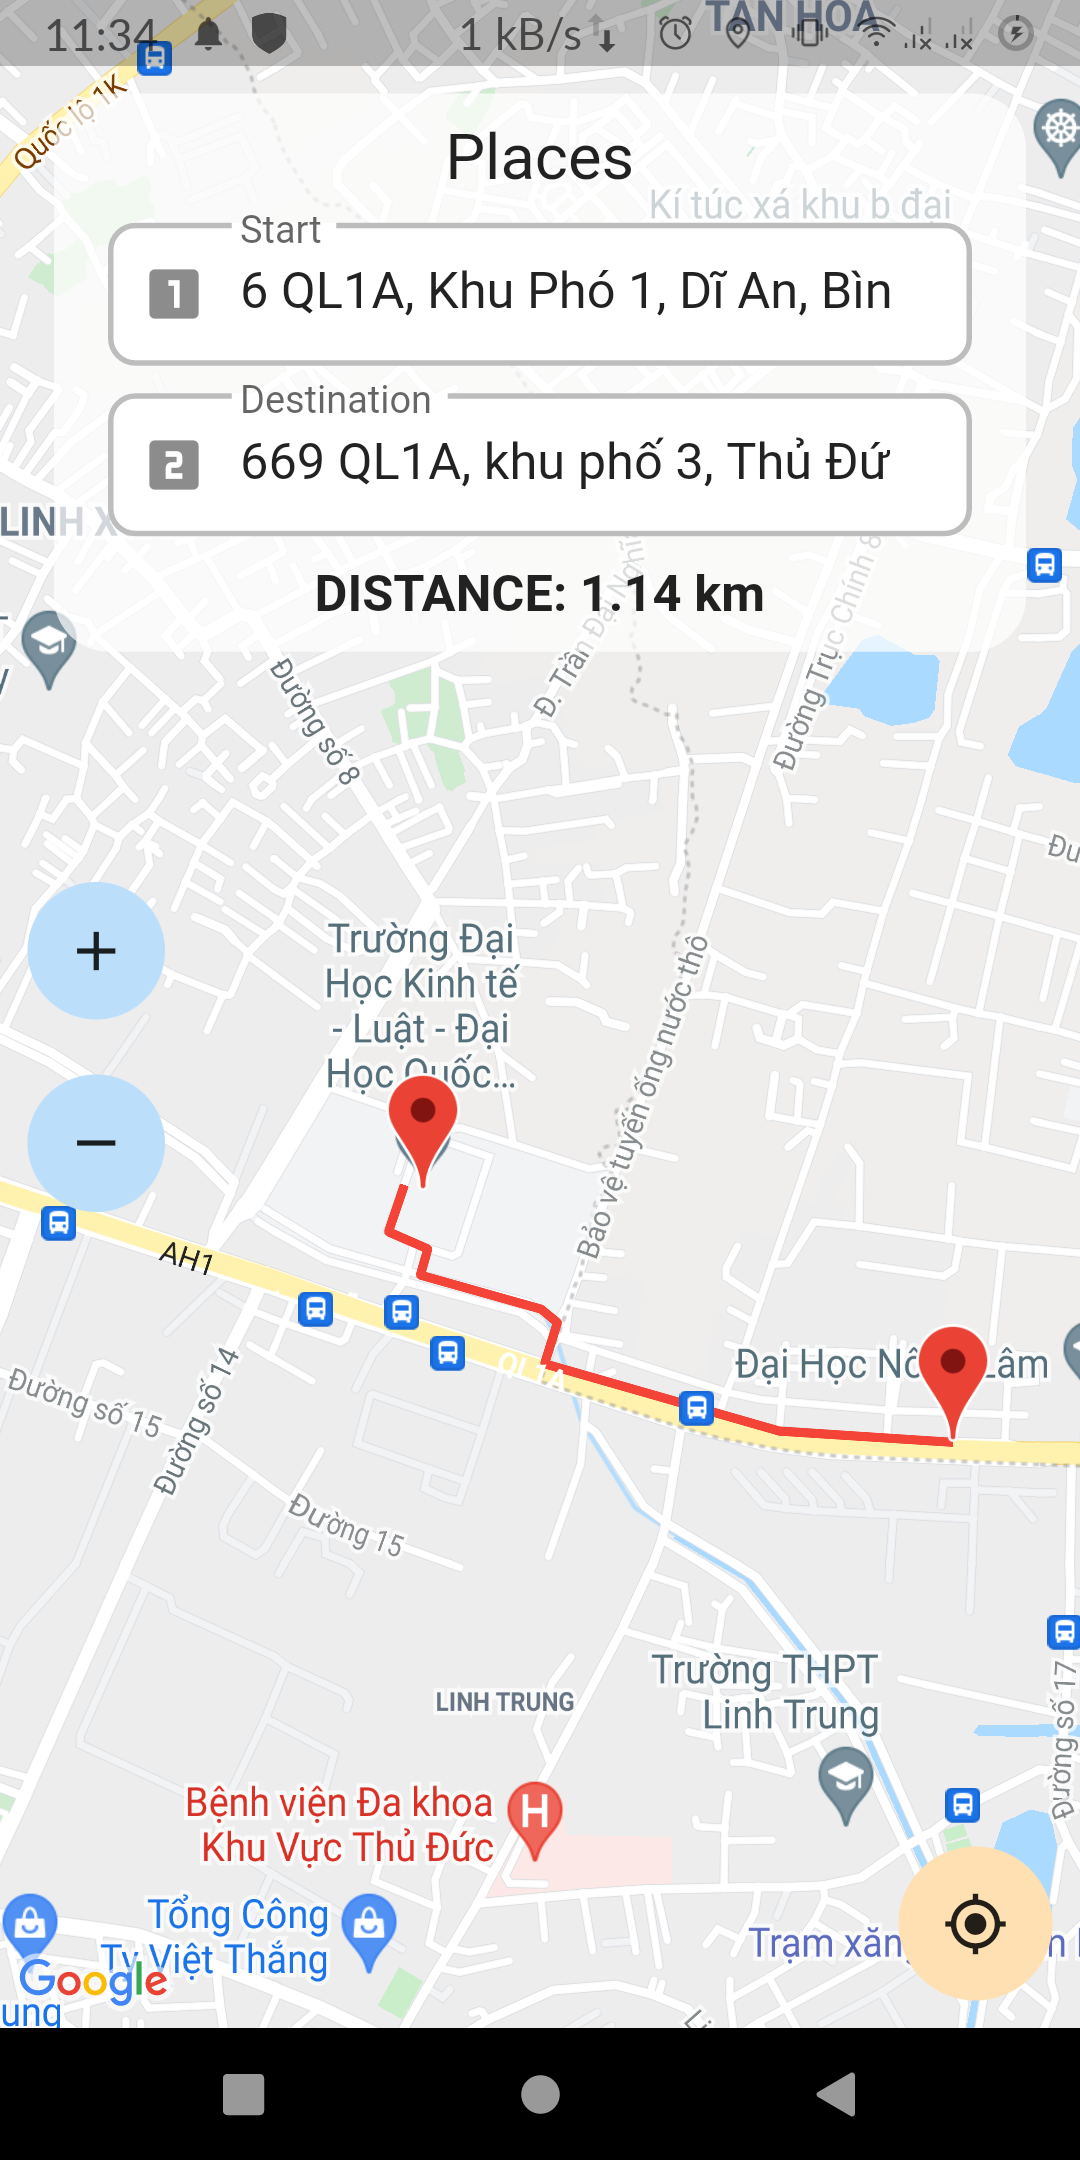
\includegraphics[width=10cm]{images/Screen-Map.png}
    \caption{Màn hình chỉ đường}
    \label{fig:screen-map}
\end{figure}

Chức năng chỉ đường từ một địa điểm đến một địa điểm xác định cho phép người dùng có thể hỏi đường bằng văn bản và giọng nói.
\begin{itemize}
    \item Hỏi đường bằng văn bản: Người dùng nhập 1 câu hỏi bằng văn bản vào ứng dụng. VD: “Đường đi từ UBND thành phố Thủ Đức đến Công An thành phố Thủ Đức”. Bấm nút gửi
    \item Hỏi đường bằng giọng nói: Người dùng ấn giữ icon ghi âm và nói 1 câu vào ứng dụng. VD: “Đường đi từ UBND thành phố Thủ Đức đến Công An thành phố Thủ Đức”
    \item Ứng dụng hiển thị câu trả lời bằng văn bản lên màn hình, chuyển văn bản thành âm thanh và phát lên.
    \item Button "Xem đường đi" dùng để chuyển sang màn hình chỉ đường của bản đồ giúp người dùng có thể xem đường đi một cách cụ thể hơn.
    \item Ở màn hình bản đồ, bạn có thể xem được đường đi cụ thể mà bạn vừa yêu cầu và khoảng cách sẽ được hiển thị lên bản đồ. Bạn có thể phóng to, thu nhỏ bản đồ và có thể xem vị trí hiện tại của mình.
\end{itemize}